%\subsection{Model Overview}

In this section, we describe our joint model for cross-lingual table linking.
%\figref{fig:overview} gives a general view of our neural network based joint model.
\figref{fig:overview} gives a general view of the model.
The reason we call it a ``joint model'' is that
the input of neural network is a mention table $X$ containing all the cells to be linked,
together with one candidate entity table $E$,
%All the mentions in the table will be linked simultaneously.
and the output stands for the relevance score $S(X, E)$.
%which indicates the probability of choosing that candidate entity table as final result.

Specifically, we first generate candidate entities of each single mention (\secref{sec:candgen}),
then we learn two different features:
the \textbf{m}ention feature and \textbf{c}ontext feature
derived from the mention-entity embedding pairs of the table (\secref{sec:cell}).
To make different representations from two language spaces compatible,
we utilize a bilingual translation matrix to transform the vector representation
from Chinese to English (\secref{sec:translation}).
Meanwhile, we learn a third feature called \textbf{coh}erence feature
only from the candidate entity table (\secref{sec:coherence}).
%We combine these three features together to calculate the overall relevance score, and finally
Finally, we discuss the prediction and parameter learning step of this task (\secref{sec:strategy}). 

\begin{figure*}
	\centering
	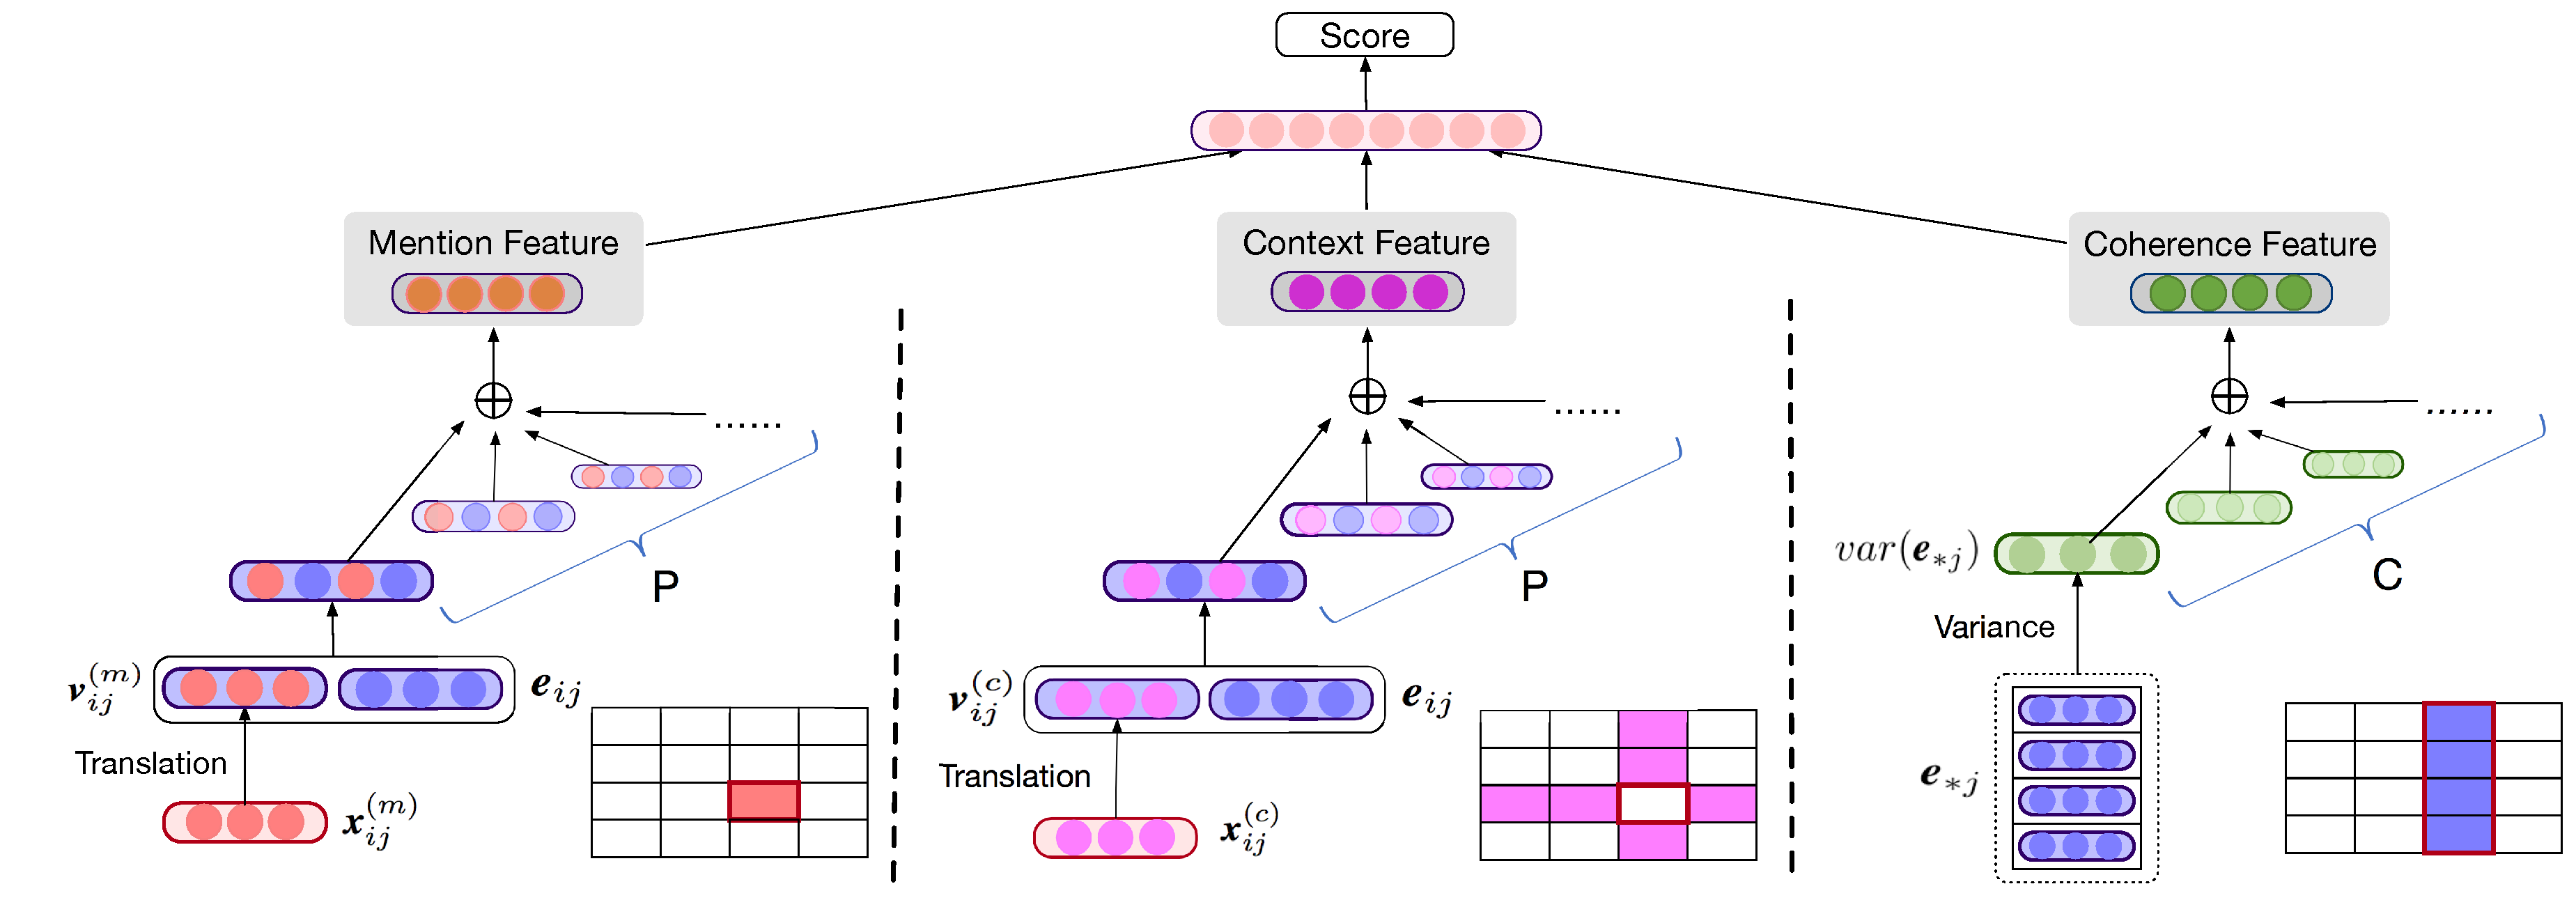
\epsfig{file=figures/overview.eps, angle=0, width=2.0\columnwidth}
	%\scalebox{0.3}{\includegraphics{overview.eps}}
	\caption{Overview of proposed neural network based joint model.}
	\label{fig:overview}
\end{figure*}
